% Options for packages loaded elsewhere
\PassOptionsToPackage{unicode}{hyperref}
\PassOptionsToPackage{hyphens}{url}
%
\documentclass[
]{article}
\usepackage{amsmath,amssymb}
\usepackage{lmodern}
\usepackage{iftex}
\ifPDFTeX
  \usepackage[T1]{fontenc}
  \usepackage[utf8]{inputenc}
  \usepackage{textcomp} % provide euro and other symbols
\else % if luatex or xetex
  \usepackage{unicode-math}
  \defaultfontfeatures{Scale=MatchLowercase}
  \defaultfontfeatures[\rmfamily]{Ligatures=TeX,Scale=1}
\fi
% Use upquote if available, for straight quotes in verbatim environments
\IfFileExists{upquote.sty}{\usepackage{upquote}}{}
\IfFileExists{microtype.sty}{% use microtype if available
  \usepackage[]{microtype}
  \UseMicrotypeSet[protrusion]{basicmath} % disable protrusion for tt fonts
}{}
\makeatletter
\@ifundefined{KOMAClassName}{% if non-KOMA class
  \IfFileExists{parskip.sty}{%
    \usepackage{parskip}
  }{% else
    \setlength{\parindent}{0pt}
    \setlength{\parskip}{6pt plus 2pt minus 1pt}}
}{% if KOMA class
  \KOMAoptions{parskip=half}}
\makeatother
\usepackage{xcolor}
\usepackage[margin=1in]{geometry}
\usepackage{color}
\usepackage{fancyvrb}
\newcommand{\VerbBar}{|}
\newcommand{\VERB}{\Verb[commandchars=\\\{\}]}
\DefineVerbatimEnvironment{Highlighting}{Verbatim}{commandchars=\\\{\}}
% Add ',fontsize=\small' for more characters per line
\usepackage{framed}
\definecolor{shadecolor}{RGB}{248,248,248}
\newenvironment{Shaded}{\begin{snugshade}}{\end{snugshade}}
\newcommand{\AlertTok}[1]{\textcolor[rgb]{0.94,0.16,0.16}{#1}}
\newcommand{\AnnotationTok}[1]{\textcolor[rgb]{0.56,0.35,0.01}{\textbf{\textit{#1}}}}
\newcommand{\AttributeTok}[1]{\textcolor[rgb]{0.77,0.63,0.00}{#1}}
\newcommand{\BaseNTok}[1]{\textcolor[rgb]{0.00,0.00,0.81}{#1}}
\newcommand{\BuiltInTok}[1]{#1}
\newcommand{\CharTok}[1]{\textcolor[rgb]{0.31,0.60,0.02}{#1}}
\newcommand{\CommentTok}[1]{\textcolor[rgb]{0.56,0.35,0.01}{\textit{#1}}}
\newcommand{\CommentVarTok}[1]{\textcolor[rgb]{0.56,0.35,0.01}{\textbf{\textit{#1}}}}
\newcommand{\ConstantTok}[1]{\textcolor[rgb]{0.00,0.00,0.00}{#1}}
\newcommand{\ControlFlowTok}[1]{\textcolor[rgb]{0.13,0.29,0.53}{\textbf{#1}}}
\newcommand{\DataTypeTok}[1]{\textcolor[rgb]{0.13,0.29,0.53}{#1}}
\newcommand{\DecValTok}[1]{\textcolor[rgb]{0.00,0.00,0.81}{#1}}
\newcommand{\DocumentationTok}[1]{\textcolor[rgb]{0.56,0.35,0.01}{\textbf{\textit{#1}}}}
\newcommand{\ErrorTok}[1]{\textcolor[rgb]{0.64,0.00,0.00}{\textbf{#1}}}
\newcommand{\ExtensionTok}[1]{#1}
\newcommand{\FloatTok}[1]{\textcolor[rgb]{0.00,0.00,0.81}{#1}}
\newcommand{\FunctionTok}[1]{\textcolor[rgb]{0.00,0.00,0.00}{#1}}
\newcommand{\ImportTok}[1]{#1}
\newcommand{\InformationTok}[1]{\textcolor[rgb]{0.56,0.35,0.01}{\textbf{\textit{#1}}}}
\newcommand{\KeywordTok}[1]{\textcolor[rgb]{0.13,0.29,0.53}{\textbf{#1}}}
\newcommand{\NormalTok}[1]{#1}
\newcommand{\OperatorTok}[1]{\textcolor[rgb]{0.81,0.36,0.00}{\textbf{#1}}}
\newcommand{\OtherTok}[1]{\textcolor[rgb]{0.56,0.35,0.01}{#1}}
\newcommand{\PreprocessorTok}[1]{\textcolor[rgb]{0.56,0.35,0.01}{\textit{#1}}}
\newcommand{\RegionMarkerTok}[1]{#1}
\newcommand{\SpecialCharTok}[1]{\textcolor[rgb]{0.00,0.00,0.00}{#1}}
\newcommand{\SpecialStringTok}[1]{\textcolor[rgb]{0.31,0.60,0.02}{#1}}
\newcommand{\StringTok}[1]{\textcolor[rgb]{0.31,0.60,0.02}{#1}}
\newcommand{\VariableTok}[1]{\textcolor[rgb]{0.00,0.00,0.00}{#1}}
\newcommand{\VerbatimStringTok}[1]{\textcolor[rgb]{0.31,0.60,0.02}{#1}}
\newcommand{\WarningTok}[1]{\textcolor[rgb]{0.56,0.35,0.01}{\textbf{\textit{#1}}}}
\usepackage{longtable,booktabs,array}
\usepackage{calc} % for calculating minipage widths
% Correct order of tables after \paragraph or \subparagraph
\usepackage{etoolbox}
\makeatletter
\patchcmd\longtable{\par}{\if@noskipsec\mbox{}\fi\par}{}{}
\makeatother
% Allow footnotes in longtable head/foot
\IfFileExists{footnotehyper.sty}{\usepackage{footnotehyper}}{\usepackage{footnote}}
\makesavenoteenv{longtable}
\usepackage{graphicx}
\makeatletter
\def\maxwidth{\ifdim\Gin@nat@width>\linewidth\linewidth\else\Gin@nat@width\fi}
\def\maxheight{\ifdim\Gin@nat@height>\textheight\textheight\else\Gin@nat@height\fi}
\makeatother
% Scale images if necessary, so that they will not overflow the page
% margins by default, and it is still possible to overwrite the defaults
% using explicit options in \includegraphics[width, height, ...]{}
\setkeys{Gin}{width=\maxwidth,height=\maxheight,keepaspectratio}
% Set default figure placement to htbp
\makeatletter
\def\fps@figure{htbp}
\makeatother
\setlength{\emergencystretch}{3em} % prevent overfull lines
\providecommand{\tightlist}{%
  \setlength{\itemsep}{0pt}\setlength{\parskip}{0pt}}
\setcounter{secnumdepth}{5}
\ifLuaTeX
  \usepackage{selnolig}  % disable illegal ligatures
\fi
\IfFileExists{bookmark.sty}{\usepackage{bookmark}}{\usepackage{hyperref}}
\IfFileExists{xurl.sty}{\usepackage{xurl}}{} % add URL line breaks if available
\urlstyle{same} % disable monospaced font for URLs
\hypersetup{
  pdftitle={An Introduction to Computing and Data for Scientists},
  hidelinks,
  pdfcreator={LaTeX via pandoc}}

\title{An Introduction to Computing and Data for Scientists}
\usepackage{etoolbox}
\makeatletter
\providecommand{\subtitle}[1]{% add subtitle to \maketitle
  \apptocmd{\@title}{\par {\large #1 \par}}{}{}
}
\makeatother
\subtitle{With R}
\author{true}
\date{2022-10-21}

\usepackage{amsthm}
\newtheorem{theorem}{Theorem}[section]
\newtheorem{lemma}{Lemma}[section]
\newtheorem{corollary}{Corollary}[section]
\newtheorem{proposition}{Proposition}[section]
\newtheorem{conjecture}{Conjecture}[section]
\theoremstyle{definition}
\newtheorem{definition}{Definition}[section]
\theoremstyle{definition}
\newtheorem{example}{Example}[section]
\theoremstyle{definition}
\newtheorem{exercise}{Exercise}[section]
\theoremstyle{definition}
\newtheorem{hypothesis}{Hypothesis}[section]
\theoremstyle{remark}
\newtheorem*{remark}{Remark}
\newtheorem*{solution}{Solution}
\begin{document}
\maketitle

{
\setcounter{tocdepth}{2}
\tableofcontents
}
\hypertarget{preface}{%
\section*{Preface}\label{preface}}
\addcontentsline{toc}{section}{Preface}

\hypertarget{introduction}{%
\section{Introduction}\label{introduction}}

\hypertarget{what-are-the-computational-and-data-sciences}{%
\subsection{What are the computational and data sciences?}\label{what-are-the-computational-and-data-sciences}}

\hypertarget{reproducibility}{%
\subsection{Reproducibility}\label{reproducibility}}

\hypertarget{setup}{%
\section{Setup}\label{setup}}

\newpage

\hypertarget{introduction-to-r}{%
\section{Introduction to R}\label{introduction-to-r}}

It is a long-standing tradition that your first program in any new programming language should simply display the message ``Hello, World!''.

In R we can use the \texttt{print()} \emph{function} to display a piece of data (such as the text \emph{Hello, World!}).

For example, we can run this line of code in R:

\begin{Shaded}
\begin{Highlighting}[]
\FunctionTok{print}\NormalTok{(}\StringTok{"Hello, World!"}\NormalTok{)}
\end{Highlighting}
\end{Shaded}

And R will return this result:

\begin{verbatim}
## [1] "Hello, World!"
\end{verbatim}

\begin{quote}
\textbf{What's happening here?}

We will learn more about the different parts of this code in this chapter,
but briefly:

\begin{itemize}
\tightlist
\item
  \texttt{print(...)} is a \textbf{function}: it takes some input ingredients (which we
  list between the brackets after the function's name), and does something
  with them.
\item
  \texttt{"Hello,\ World!"} is a string of characters (and other symbols, such as
  \texttt{!}). A \textbf{character string} is a type of data that computers can work with.
\end{itemize}
\end{quote}

\begin{exercise}
\textbf{Exercise: Try it yourself:} Open up RStudio and copy the line of code into the RStudio
Console. Then hit the key on your keyboard to run the line. You should
get back the same output as above.

Congratulations! You just ran your first program in R.
\end{exercise}

\hypertarget{data}{%
\subsection{Data}\label{data}}

The central component of everything we will be doing in R this semester is \textbf{data}. Even non-data science programs revolve around data.

At a very basic level, a computer is just a fancy calculator that adds and subtracts numbers. Even things like words and pictures are stored inside a computer as numbers.

However, we often want to work work with data that is not numbers. For example, in the last section we were able to get R to print out the sentence \emph{Hello, World!} To your computer that was just numbers flowing down wires as electrical signals. But the R programming language took care of converting our instruction into something your computer could understand.

This is the magic of programming languages! They allow us to write commands in (relatively) human-readable instructions, and then take care of translating that into the very unreadable numbers that computers work with.

R allows us to work with several ``higher-level'' types of data. These \textbf{data types} include:

\begin{itemize}
\item
  the \textbf{character} data type holds text (i.e.~letters, symbols, and the characters that represent numbers). We need to put the text inside quotation marks so that R knows where the text starts and ends: \texttt{"this\ is\ character\ data"}.

  \begin{itemize}
  \tightlist
  \item
    Note: in other programming languages this datatype is sometimes known as a ``character string'' or just a ``string''.
  \end{itemize}
\item
  the \textbf{numeric} data type holds numbers such as \texttt{0} or \texttt{12.5} (i.e.~both integers (whole numbers) and decimals). Unlike text, numbers are written \emph{without} quotation marks around them.
\item
  the \textbf{Boolean} data type holds a value that is either \texttt{TRUE} or \texttt{FALSE}. (This is sometimes also referred to as the logical data type.)
\end{itemize}

\begin{exercise}
\textbf{Exercise:} Type the number 2 into the RStudio console. Hit the key to run this line of code. What do you get back?
\end{exercise}

\hypertarget{operators}{%
\subsection{Operators}\label{operators}}

\hypertarget{combining-data-with-operators}{%
\subsubsection{Combining data with operators}\label{combining-data-with-operators}}

Okay, so now we know about data.

But data by itself is not especially useful. It just sits there until you \emph{do something} to it. In programming languages there are often many ways of doing things to data, but one of the simplest is \textbf{operators}.

Operators \emph{operate} on data. The name may sound unusual, but you are already familiar with many operators, such as \texttt{+} and \texttt{-} for adding and subtracting numbers.

\begin{exercise}
Try entering a number after the \texttt{\textgreater{}} in the Console (e.g.~1), then Enter, and see what happens.
\end{exercise}

When you hit enter, the R interpreter reads in the line, evaluates it, and returns the answer. In this case, you entered 1, so the computer thinks `Hey, it's a 1! Wow, a one! The result of 1 is\ldots{} drum roll, please\ldots{} 1!' and returns the result of this \textbf{expression}, which is a one.

Cool! But not, I confess, particularly useful. Let's fix that: next we'll add two numbers together.

\begin{exercise}
At the prompt, enter two numbers separated by a plus sign, +

\texttt{\textgreater{}\ 1\ +\ 1}

What do you get?
\end{exercise}

(Note that I've left the Console's \texttt{\textgreater{}} prompt in the example code above, but I will leave it out in future.)

Great! Let's move on and investigate operators in more depth\ldots{}

\hypertarget{operating-on-numbers}{%
\subsubsection{Operating on numbers}\label{operating-on-numbers}}

Heart surgeons operate on hearts, brain surgeons operate on brains.
You will be operating on numbers\ldots{} does that make you a data surgeon?

Here are some of the operators available to us in R:

\begin{longtable}[]{@{}ccc@{}}
\toprule()
Operator & Example & Result \\
\midrule()
\endhead
\texttt{+} & \texttt{5\ +\ 2} & \texttt{7} \\
\texttt{-} & \texttt{5\ -\ 2} & \texttt{3} \\
\texttt{*} & \texttt{5\ *\ 2} & \texttt{10} \\
\texttt{/} & \texttt{5\ /\ 2} & \texttt{2.5} \\
\texttt{\^{}} & \texttt{5\ \^{}\ 2} & \texttt{25} \\
\texttt{\%\%} & \texttt{5\ \%\%\ 2} & \texttt{1} \\
\texttt{\textless{}} & \texttt{5\ \textless{}\ 2} & \texttt{FALSE} \\
\texttt{\textgreater{}} & \texttt{5\ \textgreater{}\ 2} & \texttt{TRUE} \\
\texttt{==} & \texttt{5\ ==\ 2} & \texttt{FALSE} \\
\bottomrule()
\end{longtable}

Some of these might seem obvious, while others might be unfamiliar.
Let's go through them all and figure out what they do.

\hypertarget{the---operator}{%
\subsubsection{\texorpdfstring{The \texttt{-} operator}{The - operator}}\label{the---operator}}

\begin{exercise}
In the R Console, type \texttt{5\ -\ 2} and hit enter to run the line of code.

You probably have a good idea of what \texttt{-} does, but try changing the numbers
just to make sure!
\end{exercise}

\hypertarget{the-operator}{%
\subsubsection{\texorpdfstring{The \texttt{*} operator}{The * operator}}\label{the-operator}}

\begin{exercise}
In the R Console, type \texttt{3\ *\ 2} and hit enter to run the line of code.

What does \texttt{*} do?
\end{exercise}

\hypertarget{the-operator-1}{%
\subsubsection{\texorpdfstring{The \texttt{/} operator}{The / operator}}\label{the-operator-1}}

\begin{exercise}
In the R Console, type \texttt{3\ /\ 2} and hit enter to run the line of code.

What does \texttt{/} do? Just to be sure, try some other numbers.
\end{exercise}

\hypertarget{the-operator-2}{%
\subsubsection{\texorpdfstring{The \texttt{\^{}} operator}{The \^{} operator}}\label{the-operator-2}}

\begin{exercise}
In the R Console, type \texttt{3\ \^{}\ 2} and hit enter to run the line of code.

What does \texttt{\^{}} do? Try some other numbers like \texttt{2\ \^{}\ 3} or \texttt{16\ \^{}\ 0.5}
\end{exercise}

\hypertarget{the-operator-3}{%
\subsubsection{\texorpdfstring{The \texttt{\%\%} operator}{The \%\% operator}}\label{the-operator-3}}

\begin{exercise}
Next up, a slightly trickier one, type \texttt{3\ \%\%\ 2} and hit enter to run the line of code.

What does \texttt{\%\%} do? You will probably have to try some other numbers to figure
this one out.

If you have difficulty try also dividing the same numbers. E.g. try both
\texttt{9\ \%\%\ 4} and \texttt{9\ /\ 4}.
\end{exercise}

\hypertarget{the-and-operators}{%
\subsubsection{\texorpdfstring{The \texttt{\textless{}} and \texttt{\textgreater{}} operators}{The \textless{} and \textgreater{} operators}}\label{the-and-operators}}

\begin{exercise}
So far we have operated on numbers and got numbers back. However these next
operators will return a different type of data.

What do you get if you run \texttt{8\ \textgreater{}\ 10}?

Can you change the \texttt{8} into a number so that this expression returns \texttt{TRUE}?

Then change the \texttt{\textgreater{}} to a \texttt{\textless{}} operator (i.e.~reverse its direction).
What is the result now?
\end{exercise}

\begin{quote}
\textbf{Boolean operators}

In the previous section we learned about the Boolean data type which has only
two possible values: \texttt{TRUE} or \texttt{FALSE}.

Operators that always return a Boolean value are called Boolean operators.
The \emph{greater than} (\texttt{\textgreater{}}) and \emph{less than} (\texttt{\textless{}}) operators are examples of
Boolean operators.

You can think of Boolean operators as asking a question that can only be
be answered with either ``true'' or ``false'', such as ``Is 8 greater than 10?''
\end{quote}

\hypertarget{the-operators}{%
\subsubsection{\texorpdfstring{The \texttt{==} operators}{The == operators}}\label{the-operators}}

\begin{exercise}
Let's try another Boolean operator. What do you get if you run \texttt{8\ ==\ 10}?
What about \texttt{8\ ==\ 8}?

What do you think the \texttt{==} operator does?
\end{exercise}

\begin{quote}
\textbf{Combining comparisons}

Sometimes we want to know if one datum is greater than \textbf{or} equal
to another. You can use the Boolean operators \texttt{\textgreater{}=} for such a comparison, or
\texttt{\textless{}=} to see if something is \emph{less than or equal to} another.
\end{quote}

\hypertarget{which-operator-goes-first}{%
\subsubsection{Which operator goes first?}\label{which-operator-goes-first}}

Just like in normal math, we can do sums in R with multiple operators:

\begin{Shaded}
\begin{Highlighting}[]
\DecValTok{3} \SpecialCharTok{+} \DecValTok{5} \SpecialCharTok{/} \DecValTok{5} \SpecialCharTok{*} \DecValTok{3} \SpecialCharTok{\^{}} \DecValTok{2}
\end{Highlighting}
\end{Shaded}

In such a case, which operation do we do first?

Again, just like in regular math, some operations are always done before others. For example, all multiplication and division will be done before any addition or subtraction.

\begin{quote}
\textbf{F.Y.I.}

The order in which operators are calculated is known as \emph{operator precedence}, and you can find the precedence of any operator here: \url{https://stat.ethz.ch/R-manual/R-devel/library/base/html/Syntax.html}
\end{quote}

We can change the order of operations with parentheses: \texttt{(} and \texttt{)}. For example

\begin{Shaded}
\begin{Highlighting}[]
\DecValTok{2} \SpecialCharTok{+} \DecValTok{2} \SpecialCharTok{*} \DecValTok{5} \OtherTok{=} \DecValTok{12}
\end{Highlighting}
\end{Shaded}

whereas

\begin{Shaded}
\begin{Highlighting}[]
\NormalTok{(}\DecValTok{2} \SpecialCharTok{+} \DecValTok{2}\NormalTok{) }\SpecialCharTok{*} \DecValTok{5} \OtherTok{=} \DecValTok{20}
\end{Highlighting}
\end{Shaded}

\begin{exercise}
Modify this R code

\texttt{3\ +\ 5\ /\ 5\ *\ 2\ \^{}\ 2}

so that it performs the calculation \$rac\{3 + 5\}\{(5 imes 2) \^{} 2\}\$.

When correct, you should get the answer 0.08.
\end{exercise}

\begin{Shaded}
\begin{Highlighting}[]
\FunctionTok{grade\_result}\NormalTok{(}
  \FunctionTok{pass\_if}\NormalTok{(}\SpecialCharTok{\textasciitilde{}} \FunctionTok{identical}\NormalTok{(.result, }\FloatTok{0.08}\NormalTok{), }\StringTok{"Looks like you\textquotesingle{}re a parenthesis master!"}\NormalTok{)}
\NormalTok{)}
\end{Highlighting}
\end{Shaded}

\hypertarget{storing-and-reusing-results-with-variables}{%
\subsection{\texorpdfstring{Storing and reusing results with \emph{variables}}{Storing and reusing results with variables}}\label{storing-and-reusing-results-with-variables}}

So far we have learnt how to combine data to get different results.

We can do multiple separate calculations by putting each one on a separate line. When R reads your code, it treats everything on one line as a single expression that is separate from other lines:

\begin{Shaded}
\begin{Highlighting}[]
\DecValTok{2} \SpecialCharTok{+} \DecValTok{2}
\DecValTok{5} \SpecialCharTok{*} \DecValTok{5}
\end{Highlighting}
\end{Shaded}

This program will have two separate outputs: 4 and 25

However, after these results are shown to us, they are thrown away! All that effort just discarded\ldots{}

What if we wish to save the result of a calculation so that we can reuse it in a subsequent line?

In this case, we need to store the result in a \textbf{variable}.

\begin{exercise}
Run these two lines of code in the RStudio Console and see what result you get.

\texttt{a\ \textless{}-\ 2\ +\ 2}

\texttt{5\ *\ a}

Then take a look at the \emph{Environment} tab in the top-right pane of RStudio.
Do you see a \textbf{variable} called \texttt{a}?
Does it hold the value calculated in the first line of code or the second?
\end{exercise}

\hypertarget{the-result-of-the-assignment-operator}{%
\subsubsection{The ``result'' of the assignment operator}\label{the-result-of-the-assignment-operator}}

We store the result of an expression in a variable using the \textbf{assignment operator}: \texttt{\textless{}-}

\begin{Shaded}
\begin{Highlighting}[]
\NormalTok{variable\_name }\OtherTok{\textless{}{-}}\NormalTok{ value\_to\_be\_stored}
\end{Highlighting}
\end{Shaded}

\begin{exercise}
Run these two lines of code in the RStudio Console and see what result you get.

\texttt{2\ +\ 3}

\texttt{b\ \textless{}-\ 2\ +\ 4}

If you take another look at the \emph{Environment} tab in the top-right pane of RStudio, you should see another variable called \texttt{b}. What value does it hold?
\end{exercise}

\begin{Shaded}
\begin{Highlighting}[]
\DecValTok{2} \SpecialCharTok{+} \DecValTok{3}
\end{Highlighting}
\end{Shaded}

\begin{Shaded}
\begin{Highlighting}[]
\NormalTok{b }\OtherTok{\textless{}{-}} \DecValTok{2} \SpecialCharTok{+} \DecValTok{4}
\end{Highlighting}
\end{Shaded}

The second line of code should not print out any output when it runs.
This is because assignment has no ``result'' in the same way that a math expression does, so there is nothing to print out.

If you want to see the data that is stored in a variable, you can put the name of the variable on a line by itself:

\begin{Shaded}
\begin{Highlighting}[]
\NormalTok{some\_variable}
\end{Highlighting}
\end{Shaded}

R will evaluate this line: it will ask itself ``What is the \emph{result} of \texttt{some\_variable}'', which is just whatever value is stored in that variable.

For example,

\begin{Shaded}
\begin{Highlighting}[]
\NormalTok{c }\OtherTok{\textless{}{-}} \DecValTok{3}

\NormalTok{c}
\end{Highlighting}
\end{Shaded}

\begin{verbatim}
## [1] 3
\end{verbatim}

The other implication of this is that if you calculate something in R and do not assign the result to a variable then it will be printed out \textbf{\emph{and then forgotten}}.
So remember: if you calculate something important in R that you will need in the future, make sure that you store it in a variable.

\begin{exercise}
Type the name of one of the variables in your Environment tab in the RStudio Console (e.g.~\texttt{a}), and hit Enter to run it.

Does this return the data that you think is stored in that variable?
\end{exercise}

\begin{Shaded}
\begin{Highlighting}[]
\NormalTok{b}
\end{Highlighting}
\end{Shaded}

\begin{Shaded}
\begin{Highlighting}[]
\FunctionTok{grade\_code}\NormalTok{(}\StringTok{":)"}\NormalTok{)}
\end{Highlighting}
\end{Shaded}

\hypertarget{variables-are-variable}{%
\subsubsection{Variables are\ldots{} variable}\label{variables-are-variable}}

Variables get their name because \emph{their value can vary}. We have created the variable \texttt{b} that holds the value 6, but we can change the value of \texttt{b} and store a completely different value in it!

\begin{exercise}
Try assigning the value \texttt{7} to the variable \texttt{b} using the assignment operator \texttt{\textless{}-}.

Since we already created \texttt{b} in an earlier exercise, you should see that its value in the Environment tab updates.
\end{exercise}

\begin{Shaded}
\begin{Highlighting}[]
\NormalTok{b }\OtherTok{\textless{}{-}} \DecValTok{7}
\end{Highlighting}
\end{Shaded}

\begin{Shaded}
\begin{Highlighting}[]
\FunctionTok{grade\_result}\NormalTok{(}
  \FunctionTok{pass\_if}\NormalTok{(}\ControlFlowTok{function}\NormalTok{(x) }\FunctionTok{identical}\NormalTok{(x, }\DecValTok{7}\NormalTok{), }\StringTok{"This is a correct message."}\NormalTok{)}
\NormalTok{)}
\end{Highlighting}
\end{Shaded}

\hypertarget{when-does-assignment-happen}{%
\subsubsection{When does assignment happen}\label{when-does-assignment-happen}}

\texttt{\textless{}-} is an operator, just like \texttt{+} or \texttt{*}. As such, it has a \emph{precedence}: it will happen before some operators but after others.

However, it turns out that the \texttt{\textless{}-} precedence is \href{https://stat.ethz.ch/R-manual/R-devel/library/base/html/Syntax.html}{extremely low} - i.e.~it will happen after the result of all the other operators on that line of code have been calculated.

So, when you write:

\begin{Shaded}
\begin{Highlighting}[]
\NormalTok{a }\OtherTok{\textless{}{-}} \DecValTok{2} \SpecialCharTok{+} \DecValTok{4}
\end{Highlighting}
\end{Shaded}

\ldots you are essentially doing this:

\begin{Shaded}
\begin{Highlighting}[]
\NormalTok{a }\OtherTok{\textless{}{-}}\NormalTok{ (}\DecValTok{2} \SpecialCharTok{+} \DecValTok{4}\NormalTok{)}
\end{Highlighting}
\end{Shaded}

\hypertarget{how-r-works}{%
\subsection{How R works}\label{how-r-works}}

R is an \emph{interpreted programming language}.

That is a fancy way of saying that R runs (i.e.~``interprets'') every line of code one at a time.

So far we have written a line of code and then run it. In a couple of exercises you may have run multiple lines of code where one line depended on a result from a previous line. However, R completely finished running the first line before moving onto the next one.

When R \emph{interprets} a line of code, it figures out how to convert your human-readable code into computer-readable instructions (which are a series of 0s and 1s, since a computer is basically a bunch of wires that can either have an electrical current flowing down them (which we denote as 1) or not (0)).

Because R is interpreted line-by-line, it is an ideal programming language for exploring and analyzing scientific data, where we typically figure out what to do next as we go along!

We will soon be learning how to write multiple lines of R code in a file and then run them from the file. However, even when R runs code from a file, it still figures out how to run it one line at a time.

\begin{quote}
\textbf{Compiled Programming Languages}

Not every programming language is interpreted like R. Some are \emph{compiled}.

This means that you write all your code in a file, and then turn all of it into computer-readable instructions at once. This step is called \emph{compilation} and can take a long time (up to hours for large programs in some languages!). It is typically slower to write programs in a compiled language because of this extra step.

The main advantage of a compiled programming language is that your computer can figure out how to optimize all the lines of code so that they run extremely fast.

Famous examples of compiled programming languages are Java and C++.
\end{quote}

\hypertarget{more-about-data}{%
\subsection{More about data}\label{more-about-data}}

\hypertarget{boolean-data-revisted}{%
\subsubsection{Boolean data revisted}\label{boolean-data-revisted}}

At the start of this chapter we mentioned that there is a type of data in R, called Boolean data, that can have one of two values: \texttt{TRUE} or \texttt{FALSE}.

Then in the section on operators we saw that some operators (those that do comparisons) would give a \texttt{TRUE}/\texttt{FALSE} result even when the input data was not Boolean. For example,

\begin{Shaded}
\begin{Highlighting}[]
\DecValTok{2} \SpecialCharTok{==} \DecValTok{2}
\end{Highlighting}
\end{Shaded}

\begin{verbatim}
## [1] TRUE
\end{verbatim}

because 2 is equal to 2 (i.e.~this is a \emph{true} expression).

The value \texttt{2} is an example of \emph{numeric} data. However, the result \texttt{TRUE} is an example of \textbf{Boolean} data.

A Boolean value can only have one of two values (i.e.~TRUE and FALSE). We often get a Boolean value when we do comparisons (e.g.~checking if two values are equal, or if one is greater than the other).

Just as with numeric data, we can store a Boolean value in a variable, e.g.~\texttt{d\ \textless{}-\ FALSE}.

\begin{exercise}
Assign the value \texttt{TRUE} to a variable called \texttt{d}.
\end{exercise}

\begin{Shaded}
\begin{Highlighting}[]
\NormalTok{ d }\OtherTok{\textless{}{-}} \ConstantTok{TRUE}
\end{Highlighting}
\end{Shaded}

\begin{Shaded}
\begin{Highlighting}[]
\FunctionTok{grade\_code}\NormalTok{(}\StringTok{":)"}\NormalTok{)}
\end{Highlighting}
\end{Shaded}

\hypertarget{combining-pieces-of-data}{%
\subsubsection{Combining pieces of data}\label{combining-pieces-of-data}}

So far we have looked at pieces of data by themselves:

\begin{Shaded}
\begin{Highlighting}[]
\NormalTok{a }\OtherTok{\textless{}{-}} \DecValTok{1}
\NormalTok{b }\OtherTok{\textless{}{-}} \StringTok{"Hello!"}
\NormalTok{c }\OtherTok{\textless{}{-}} \ConstantTok{TRUE}
\FunctionTok{print}\NormalTok{(a)}
\end{Highlighting}
\end{Shaded}

\begin{verbatim}
## [1] 1
\end{verbatim}

\begin{Shaded}
\begin{Highlighting}[]
\FunctionTok{print}\NormalTok{(b)}
\end{Highlighting}
\end{Shaded}

\begin{verbatim}
## [1] "Hello!"
\end{verbatim}

\begin{Shaded}
\begin{Highlighting}[]
\FunctionTok{print}\NormalTok{(c)}
\end{Highlighting}
\end{Shaded}

\begin{verbatim}
## [1] TRUE
\end{verbatim}

But what about if we want to combine multiple pieces of data together?

R includes several types of \emph{container} that can hold multiple pieces of data. We can then refer to that container by a single variable. For example, instead of the three variables above, we can create a \textbf{list} object that holds all three values:

\begin{Shaded}
\begin{Highlighting}[]
\NormalTok{l }\OtherTok{\textless{}{-}} \FunctionTok{list}\NormalTok{(}\DecValTok{1}\NormalTok{, }\StringTok{"Hello!"}\NormalTok{, }\ConstantTok{TRUE}\NormalTok{)}
\NormalTok{l}
\end{Highlighting}
\end{Shaded}

\begin{verbatim}
## [[1]]
## [1] 1
## 
## [[2]]
## [1] "Hello!"
## 
## [[3]]
## [1] TRUE
\end{verbatim}

We create a list using \texttt{list()}. Every value in the list goes inside the parentheses, separated by commas.

\begin{exercise}
Create a list holding 4 values (in this order): 10, ``z'', FALSE, -0.1*10
\end{exercise}

\begin{Shaded}
\begin{Highlighting}[]
\FunctionTok{list}\NormalTok{(}\DecValTok{10}\NormalTok{, }\StringTok{"z"}\NormalTok{, }\ConstantTok{FALSE}\NormalTok{, }\SpecialCharTok{{-}}\FloatTok{0.1}\SpecialCharTok{*}\DecValTok{10}\NormalTok{)}
\end{Highlighting}
\end{Shaded}

\begin{Shaded}
\begin{Highlighting}[]
\FunctionTok{grade\_code}\NormalTok{(}\StringTok{":)"}\NormalTok{)}
\end{Highlighting}
\end{Shaded}

\hypertarget{vectors}{%
\subsubsection{Vectors}\label{vectors}}

Lists can hold data of different types. For example, our list \texttt{l} holds a number, a character string, and a Boolean value.

An alternative container in R is a \textbf{vector}. Vectors can also hold multiple pieces of data, but unlike a list, \emph{all the data in a vector must be the same type of data}. For example, a vector could contain all numbers, or all characters, but not a mix of the two.

We create a vector with \texttt{c()}:

\begin{Shaded}
\begin{Highlighting}[]
\FunctionTok{c}\NormalTok{(}\DecValTok{1}\NormalTok{,}\DecValTok{2}\NormalTok{,}\DecValTok{3}\NormalTok{)}
\end{Highlighting}
\end{Shaded}

\begin{verbatim}
## [1] 1 2 3
\end{verbatim}

\begin{exercise}
Create a vector holding 3 character strings (in this order): ``This'', ``is a'', ``vector!''
\end{exercise}

\begin{Shaded}
\begin{Highlighting}[]
\FunctionTok{c}\NormalTok{(}\StringTok{"This"}\NormalTok{, }\StringTok{"is a"}\NormalTok{, }\StringTok{"vector!"}\NormalTok{)}
\end{Highlighting}
\end{Shaded}

\begin{Shaded}
\begin{Highlighting}[]
\FunctionTok{grade\_code}\NormalTok{(}\StringTok{":)"}\NormalTok{)}
\end{Highlighting}
\end{Shaded}

\begin{quote}
You might be wondering what the numbers in square brackets at the start of each line in the output mean? E.g. \texttt{{[}1{]}}

These tell us where abouts in the vector we are. The number indicates the position in the vector of the first element displayed on that line.

For example, the \texttt{{[}1{]}} at the start of the line (before ``Introduction'') shows that ``Introduction'' is the first element in this vector.
\#\#\# Operations on vectors
\end{quote}

We can use operators on more complicated data structures just as we did on the simpler data types. For example, we can add 2 vectors together:

\begin{Shaded}
\begin{Highlighting}[]
\NormalTok{v1 }\OtherTok{\textless{}{-}} \FunctionTok{c}\NormalTok{(}\DecValTok{1}\NormalTok{,}\DecValTok{2}\NormalTok{,}\DecValTok{3}\NormalTok{)}
\NormalTok{v2 }\OtherTok{\textless{}{-}} \FunctionTok{c}\NormalTok{(}\DecValTok{4}\NormalTok{,}\DecValTok{5}\NormalTok{,}\DecValTok{6}\NormalTok{)}
\NormalTok{v1 }\SpecialCharTok{+}\NormalTok{ v2}
\end{Highlighting}
\end{Shaded}

\begin{verbatim}
## [1] 5 7 9
\end{verbatim}

As you can see, the individual elements are added together.

\begin{exercise}
What happens if you add two vectors of different lengths? For example, run this code and see what happens:
\end{exercise}

\begin{Shaded}
\begin{Highlighting}[]
\NormalTok{v3 }\OtherTok{\textless{}{-}} \FunctionTok{c}\NormalTok{(}\DecValTok{10}\NormalTok{, }\DecValTok{20}\NormalTok{, }\DecValTok{30}\NormalTok{, }\DecValTok{40}\NormalTok{, }\DecValTok{50}\NormalTok{)}
\NormalTok{v4 }\OtherTok{\textless{}{-}} \FunctionTok{c}\NormalTok{(}\DecValTok{1}\NormalTok{, }\DecValTok{2}\NormalTok{)}
\NormalTok{v3 }\SpecialCharTok{+}\NormalTok{ v4}
\end{Highlighting}
\end{Shaded}

\begin{verbatim}
## Warning in v3 + v4: longer object length is not a multiple of shorter object
## length
\end{verbatim}

What happens when you add two \texttt{v3} and \texttt{v4}?

\begin{itemize}
\tightlist
\item
  The 2 elements of v3 are added to the first 2 elements of v4, and the rest of v4 is unchanged.
\item
  v4 is repeated to match the length of v3 before they are added.
\item
  R guesses values for the remaining values of v3 so that the two vectors are the same length.
\end{itemize}

\begin{Shaded}
\begin{Highlighting}[]
\NormalTok{v3 }\OtherTok{\textless{}{-}} \FunctionTok{c}\NormalTok{(}\DecValTok{10}\NormalTok{, }\DecValTok{20}\NormalTok{, }\DecValTok{30}\NormalTok{, }\DecValTok{40}\NormalTok{, }\DecValTok{50}\NormalTok{)}
\NormalTok{v4 }\OtherTok{\textless{}{-}} \FunctionTok{c}\NormalTok{(}\DecValTok{1}\NormalTok{, }\DecValTok{2}\NormalTok{)}
\NormalTok{v3 }\SpecialCharTok{+}\NormalTok{ v4}
\end{Highlighting}
\end{Shaded}

\hypertarget{expressions-and-how-they-are-evaluated}{%
\subsection{Expressions and how they are evaluated}\label{expressions-and-how-they-are-evaluated}}

TODO

\begin{itemize}
\tightlist
\item
  Expressions and how they are evaluated. Lines and files.
\end{itemize}

\hypertarget{functions}{%
\subsection{Functions}\label{functions}}

Perhaps, keen mathematician that you are, you want to calculate the length of the hypotenuse of a triangle. Dredging up memories of early math classes, you will doubtless recall Pythagoras's theorem that the hypotenuse (the long side) of triangle is given by:

\(c = \sqrt{a^2 + b^2}\)

(\(c\) is the hypotenuse {[}long side{]} and \(a\) and \(b\) are the short sides.)

\begin{exercise}
Let's say we have a triangle where the shorter sides (a \& b) are 3 and 4 units long. Can you calculate the length of side c in R using just the operators from the first section?

\emph{Hint \#1:} The square root is equal to the 0.5 power of a number: \texttt{4\ \^{}\ 0.5\ =\ 2}

\emph{Hint \#2:} Just like in regular math equations, R will calculate some operators before others. For example it will do all multiplications before any additions. However, just like in regular math, we can change the order of operations by wrapping parts of our calculation in parentheses: \texttt{(...)}
\end{exercise}

Did you get the answer 5? Fantastic!

\begin{Shaded}
\begin{Highlighting}[]
\FunctionTok{grade\_conditions}\NormalTok{(}
  \FunctionTok{pass\_if}\NormalTok{(}\SpecialCharTok{\textasciitilde{}}\NormalTok{ .result }\SpecialCharTok{==} \FunctionTok{sqrt}\NormalTok{(}\DecValTok{10}\SpecialCharTok{\^{}}\DecValTok{2} \SpecialCharTok{+} \DecValTok{20}\SpecialCharTok{\^{}}\DecValTok{2}\NormalTok{))}
\NormalTok{)}
\end{Highlighting}
\end{Shaded}

\hypertarget{re-useable-code-functions}{%
\subsubsection{Re-useable code = functions}\label{re-useable-code-functions}}

What's that? Another complaint? You have to write out this long expression every time you need the hypotenuse of a triangle? (No doubt this is a frequent chore in your day-to-day life.)

Again, there is a solution! R allows us to save pieces of code in variables. Yes, you heard that right: variables don't just have to store data, they can also store code!

These stored, reusable sections of code are called \textbf{functions}.

For example, you could create a function to calculate the sum of two numbers:

\begin{verbatim}
adder <- function(number1, number2) {
    result <- number1 + number2
    return(result)
}
\end{verbatim}

Entering these 4 lines at the console prompt will be slow and error-prone, so let's try something different.

Click on the ``File'' menu at the top of RStudio. Select ``New File'' and then ``R Script''. A blank editor window should appear in a new pane above the console.

Copy the adder function from the previous page into this empty script. Then press ``Control + Alt + R'' on your keyboard (simultaneously). This will run the contents of your script all at once.

If successful, you should see that \texttt{adder} appears in the Environment pane under a new section called \emph{Functions}.

How do we use our adder function? Go back to the console, and type something like this:

\begin{quote}
adder(3, 5)
\end{quote}

If your function is working correctly you should get the result of the 2 numbers that you entered inside the braces.

Let's take another look at the adder function to understand what's going on:

\begin{verbatim}
adder <- function(number1, number2) {
    result <- number1 + number2
    return(result)
}
\end{verbatim}

\textbf{Line 1:} The first line creates a new function with the \texttt{function} keyword and saves it to the name \texttt{adder} using the assignment operator \texttt{\textless{}-}, just as we did for variables.

After \texttt{function} are a pair of parentheses. Inside these, we put a list of the parameters that the function can take, separated by commas. In this case, our adder function has two paramters (the numbers to add together). We are going to give these numbers the temporary names \texttt{number1} and \texttt{number2} (creative, I know). We will use these parameter names inside the function to refer to these two numbers.

We end the line with an opening curly bracket \texttt{\{} to indicate that the code that follows is part of the function.

\textbf{Line 2:} This is the meat of our adder function. We add our two number paramters together and store them in a variable called \texttt{result}. Its important to note that \texttt{result} only exists inside the curly brackets of the adder function (i.e.~it vanishes after the function has finished).

\textbf{Line 3:} Here we specify what the function is should return: in this case we want to return the \texttt{result} variable.

\textbf{Line 4:} We signal the end of the function with a closing curly bracket (matching the one from the end of line 1).

You might object (and not without reason) that our \texttt{adder} function is a very trivial example. Wouldn't it just be easier to use the \texttt{+} operator?

Yes, it would! So let's look at a more complicated function.

We can create a function to calculate the hypotenuse like this:

\begin{Shaded}
\begin{Highlighting}[]
\NormalTok{hypotenuse }\OtherTok{\textless{}{-}} \ControlFlowTok{function}\NormalTok{(a, b) \{}
\NormalTok{  c }\OtherTok{\textless{}{-}}\NormalTok{ (a}\SpecialCharTok{\^{}}\DecValTok{2} \SpecialCharTok{+}\NormalTok{ b}\SpecialCharTok{\^{}}\DecValTok{2}\NormalTok{)}\SpecialCharTok{\^{}}\FloatTok{0.5}
  \FunctionTok{return}\NormalTok{(c)}
\NormalTok{\}}
\end{Highlighting}
\end{Shaded}

Then we can use this \texttt{hypotenuse} function as many times as we like. For example calculate the hypotenuse of a triangle with sides of length 3 and 4, we would run:

\begin{Shaded}
\begin{Highlighting}[]
\FunctionTok{hypotenuse}\NormalTok{(}\DecValTok{3}\NormalTok{, }\DecValTok{4}\NormalTok{)}
\end{Highlighting}
\end{Shaded}

\begin{verbatim}
## [1] 5
\end{verbatim}

\begin{exercise}
Use the \texttt{hypotenuse()} function to calculate the area of a triangle with sides of length 3 and 4.

\emph{Hint:} Try changing the numbers inside the parentheses after \texttt{hypotenuse}.
\end{exercise}

Did you get the answer 5? Fantastic!

\begin{Shaded}
\begin{Highlighting}[]
\NormalTok{hypotenuse }\OtherTok{\textless{}{-}} \ControlFlowTok{function}\NormalTok{(a, b) \{}
\NormalTok{  c }\OtherTok{\textless{}{-}}\NormalTok{ (a}\SpecialCharTok{\^{}}\DecValTok{2} \SpecialCharTok{+}\NormalTok{ b}\SpecialCharTok{\^{}}\DecValTok{2}\NormalTok{)}\SpecialCharTok{\^{}}\FloatTok{0.5}
  \FunctionTok{return}\NormalTok{(c)}
\NormalTok{\}}
\end{Highlighting}
\end{Shaded}

\begin{Shaded}
\begin{Highlighting}[]
\FunctionTok{grade\_conditions}\NormalTok{(}
  \FunctionTok{pass\_if}\NormalTok{(}\SpecialCharTok{\textasciitilde{}}\NormalTok{ .result }\SpecialCharTok{==} \FunctionTok{sqrt}\NormalTok{(}\DecValTok{3}\SpecialCharTok{\^{}}\DecValTok{2} \SpecialCharTok{+} \DecValTok{4}\SpecialCharTok{\^{}}\DecValTok{2}\NormalTok{))}
\NormalTok{)}
\end{Highlighting}
\end{Shaded}

\hypertarget{how-the-hypotenuse-function-works}{%
\subsubsection{\texorpdfstring{How the \texttt{hypotenuse} function works}{How the hypotenuse function works}}\label{how-the-hypotenuse-function-works}}

There are a few things to note about this code:

\begin{itemize}
\tightlist
\item
  We tell R that we are creating a reusable function using the \texttt{function} keyword.
\item
  \texttt{function} is followed by parentheses \texttt{(...)} that contain \textbf{parameters}. Parameters are the names that we give to the input data to the function.

  \begin{itemize}
  \tightlist
  \item
    For example, above we created two parameters: \texttt{a} and \texttt{b}
  \item
    You can have as many parameters as you want in a function, from zero on up. They must be separated by commas.
  \end{itemize}
\item
  The reusable code goes inside a pair of curly brackets \texttt{\{...\}}

  \begin{itemize}
  \tightlist
  \item
    We can now use the function's parameters in this code (e.g.~\texttt{a} and \texttt{b}). Essentially we temporarily create new variables with the parameter names (but these are)
  \end{itemize}
\item
  At the end of the function we can return a particular result with \texttt{return(...)} - just replace the dots with a value or
\item
  We store the function in a name with the assignment operator \texttt{\textless{}-} (just like we did with variables)
\item
  When we want to run the code, we write the function name followed by parentheses, with any arguments inside the parentheses (separated by commas)
\end{itemize}

\begin{exercise}
Replace the blanks to create a function to calculate the \emph{area of a triangle} instead. Save this function as \texttt{triangle\_area}.

\_\_\_\_\_\_\_ \textless- function(a, b) \{
area \textless- \_\_\_\_\_\_\_
return(area)
\}

\emph{Hint:} The area of a triangle is \(0.5 imes a imes b\).
\end{exercise}

\begin{Shaded}
\begin{Highlighting}[]
\NormalTok{\_\_\_\_\_\_\_ }\OtherTok{\textless{}{-}} \ControlFlowTok{function}\NormalTok{(a, b) \{}
\NormalTok{  area }\OtherTok{\textless{}{-}}\NormalTok{ \_\_\_\_\_\_\_}
  \FunctionTok{return}\NormalTok{(area)}
\NormalTok{\}}
\end{Highlighting}
\end{Shaded}

\begin{Shaded}
\begin{Highlighting}[]
\FunctionTok{grade\_conditions}\NormalTok{(}
  \FunctionTok{pass\_if}\NormalTok{(}\SpecialCharTok{\textasciitilde{}} \FunctionTok{identical}\NormalTok{(}\FunctionTok{.result}\NormalTok{(}\DecValTok{4}\NormalTok{,}\DecValTok{5}\NormalTok{), }\DecValTok{10}\NormalTok{)),}
  \FunctionTok{pass\_if}\NormalTok{(}\SpecialCharTok{\textasciitilde{}} \FunctionTok{identical}\NormalTok{(}\FunctionTok{.result}\NormalTok{(}\DecValTok{10}\NormalTok{,}\DecValTok{20}\NormalTok{), }\DecValTok{100}\NormalTok{))}
\NormalTok{)}
\end{Highlighting}
\end{Shaded}

\newpage

\hypertarget{visualizing-data}{%
\section{Visualizing Data}\label{visualizing-data}}

In this chapter we will learn how to make simple graphs using R.

\hypertarget{visualization-principles}{%
\subsection{Visualization principles}\label{visualization-principles}}

This video will introduce you to the importance of visualization in data science, and how it can be used effectively (or ineffectively).

Slides: \href{https://gmuedu-my.sharepoint.com/:b:/g/personal/dwhite34_gmu_edu/ETyT0aRqt6tHspWXcGyumEgBG6K79TUuaN0mWTLsaiOySA?e=KkfEsO}{PDF}

\begin{quote}
A picture is worth thousand words\ldots{}
\end{quote}

\ldots and a good graph is clearer than a table of data.

In pre-modern times, our ancestors did not have to worry about tables of data (or words). But they did have to interpret patterns in what they saw.

We are stuck with the same brains, and so while a column of numbers doesn't mean much, if we can transform that column into a picture then patterns can become much clearer.

Example: Challenger Disaster

In 1985 the

\begin{Shaded}
\begin{Highlighting}[]
\FunctionTok{library}\NormalTok{(tidyverse)}
\end{Highlighting}
\end{Shaded}

\begin{verbatim}
## -- Attaching packages --------------------------------------- tidyverse 1.3.1 --
\end{verbatim}

\begin{verbatim}
## v ggplot2 3.3.6     v purrr   0.3.4
## v tibble  3.1.8     v dplyr   1.0.9
## v tidyr   1.2.0     v stringr 1.4.0
## v readr   2.1.2     v forcats 0.5.1
\end{verbatim}

\begin{verbatim}
## -- Conflicts ------------------------------------------ tidyverse_conflicts() --
## x dplyr::filter() masks stats::filter()
## x dplyr::lag()    masks stats::lag()
\end{verbatim}

\begin{Shaded}
\begin{Highlighting}[]
\NormalTok{tufte\_data }\OtherTok{\textless{}{-}} \FunctionTok{tibble}\NormalTok{(}
  \AttributeTok{flight =} \FunctionTok{c}\NormalTok{(}\StringTok{"51{-}C"}\NormalTok{, }\StringTok{"41{-}B"}\NormalTok{, }\StringTok{"61{-}C"}\NormalTok{, }\StringTok{"41{-}C"}\NormalTok{, }\StringTok{"1"}\NormalTok{, }\StringTok{"6"}\NormalTok{, }\StringTok{"51{-}A"}\NormalTok{, }\StringTok{"51{-}D"}\NormalTok{, }\StringTok{"5"}\NormalTok{, }\StringTok{"3"}\NormalTok{, }\StringTok{"2"}\NormalTok{, }\StringTok{"9"}\NormalTok{, }\StringTok{"41{-}D"}\NormalTok{, }\StringTok{"51{-}G"}\NormalTok{, }\StringTok{"7"}\NormalTok{, }\StringTok{"8"}\NormalTok{, }\StringTok{"51{-}B"}\NormalTok{, }\StringTok{"61{-}A"}\NormalTok{, }\StringTok{"51{-}I"}\NormalTok{, }\StringTok{"61{-}B"}\NormalTok{, }\StringTok{"41{-}G"}\NormalTok{, }\StringTok{"51{-}J"}\NormalTok{, }\StringTok{"4"}\NormalTok{, }\StringTok{"51{-}F"}\NormalTok{),}
  \AttributeTok{temperature =} \FunctionTok{c}\NormalTok{(}\DecValTok{51}\NormalTok{,}\DecValTok{57}\NormalTok{,}\DecValTok{58}\NormalTok{,}\DecValTok{63}\NormalTok{,}\DecValTok{66}\NormalTok{,}\DecValTok{67}\NormalTok{,}\DecValTok{67}\NormalTok{,}\DecValTok{67}\NormalTok{,}\DecValTok{68}\NormalTok{,}\DecValTok{69}\NormalTok{,}\DecValTok{70}\NormalTok{,}\DecValTok{70}\NormalTok{,}\DecValTok{70}\NormalTok{,}\DecValTok{70}\NormalTok{,}\DecValTok{72}\NormalTok{,}\DecValTok{73}\NormalTok{,}\DecValTok{75}\NormalTok{,}\DecValTok{76}\NormalTok{,}\DecValTok{76}\NormalTok{,}\DecValTok{76}\NormalTok{,}\DecValTok{78}\NormalTok{,}\DecValTok{79}\NormalTok{,}\DecValTok{80}\NormalTok{,}\DecValTok{81}\NormalTok{),}
  \AttributeTok{damage =} \FunctionTok{c}\NormalTok{(}\DecValTok{11}\NormalTok{,}\DecValTok{4}\NormalTok{,}\DecValTok{4}\NormalTok{,}\DecValTok{2}\NormalTok{,}\DecValTok{0}\NormalTok{,}\DecValTok{0}\NormalTok{,}\DecValTok{0}\NormalTok{,}\DecValTok{0}\NormalTok{,}\DecValTok{0}\NormalTok{,}\DecValTok{0}\NormalTok{,}\DecValTok{4}\NormalTok{,}\DecValTok{0}\NormalTok{,}\DecValTok{0}\NormalTok{,}\DecValTok{4}\NormalTok{,}\DecValTok{0}\NormalTok{,}\DecValTok{0}\NormalTok{,}\DecValTok{0}\NormalTok{,}\DecValTok{0}\NormalTok{,}\DecValTok{0}\NormalTok{,}\DecValTok{0}\NormalTok{,}\DecValTok{0}\NormalTok{,}\DecValTok{0}\NormalTok{,}\ConstantTok{NA}\NormalTok{,}\DecValTok{0}\NormalTok{)}
\NormalTok{)}
\NormalTok{tufte\_data }\SpecialCharTok{\%\textgreater{}\%}
  \FunctionTok{ggplot}\NormalTok{(}\FunctionTok{aes}\NormalTok{(temperature, damage)) }\SpecialCharTok{+}
  \FunctionTok{geom\_point}\NormalTok{() }\SpecialCharTok{+}
  \FunctionTok{geom\_smooth}\NormalTok{() }\SpecialCharTok{+}
  \FunctionTok{xlim}\NormalTok{(}\DecValTok{20}\NormalTok{,}\DecValTok{90}\NormalTok{)}
\end{Highlighting}
\end{Shaded}

\begin{verbatim}
## `geom_smooth()` using method = 'loess' and formula 'y ~ x'
\end{verbatim}

\begin{verbatim}
## Warning: Removed 1 rows containing non-finite values (stat_smooth).
\end{verbatim}

\begin{verbatim}
## Warning: Removed 1 rows containing missing values (geom_point).
\end{verbatim}

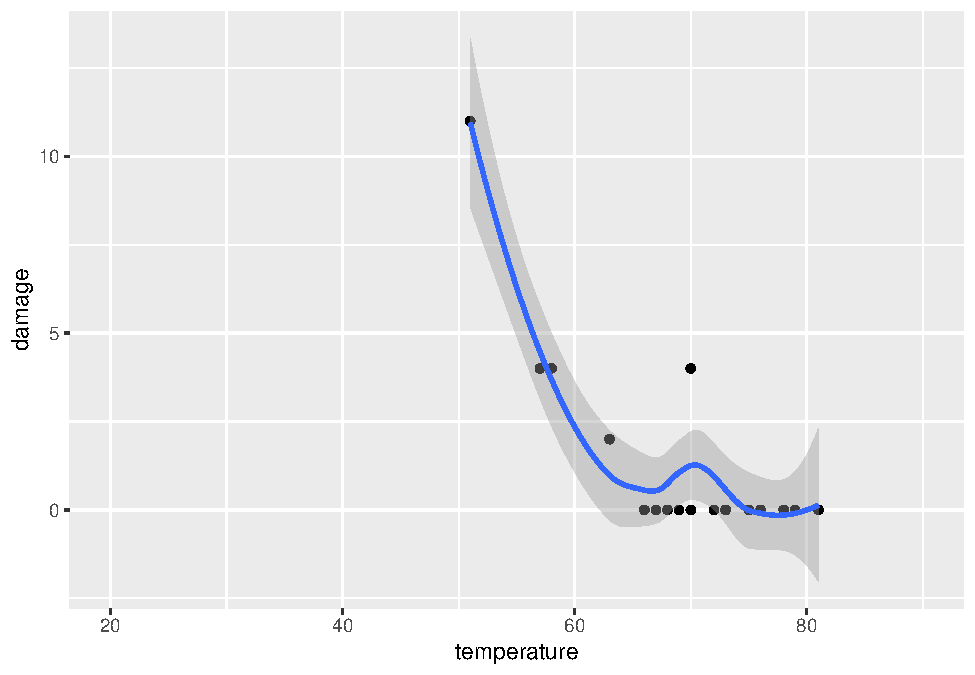
\includegraphics{intro_to_cds_files/figure-latex/unnamed-chunk-88-1.pdf}

Pictures of data are called ``graphs''.

There are many ways that we can visualize the same data. Some of these ways \emph{may} be good, but many of them \emph{will} be bad.

\hypertarget{data-overview}{%
\subsection{Data Overview}\label{data-overview}}

Before we begin to make our own graphs, we need to learn some terminology for describing the underlying data.

Slides: \href{https://gmuedu-my.sharepoint.com/:b:/g/personal/dwhite34_gmu_edu/ETqhI64qDaFGja02KJaA_usBe0iEVyOhjM5kH7ENZswmsg?e=mg4B0G}{PDF}

TBA: written version

\hypertarget{the-plot-function}{%
\subsection{\texorpdfstring{The \texttt{plot()} function}{The plot() function}}\label{the-plot-function}}

TBD

\hypertarget{one-variable-histograms-and-bar-charts}{%
\subsection{One variable: histograms and bar charts}\label{one-variable-histograms-and-bar-charts}}

TBD

\hypertarget{two-variables-scatter-plots}{%
\subsection{Two variables: scatter plots}\label{two-variables-scatter-plots}}

TBD

\hypertarget{trends-line-graphs}{%
\subsection{Trends: line graphs}\label{trends-line-graphs}}

TBD

\hypertarget{improving-your-graphs}{%
\subsection{Improving your graphs}\label{improving-your-graphs}}

TBD

\newpage

\hypertarget{wrangling-data}{%
\section{Wrangling Data}\label{wrangling-data}}

In this chapter we will learn how to manipulate and transform tables of data.

\hypertarget{wrangling-overview}{%
\subsection{Wrangling overview}\label{wrangling-overview}}

Slides: \href{https://drive.google.com/file/d/1LssVpGMhlblGewJtwO3NgdSZO-FF0uQQ}{PDF}

\hypertarget{the-dplyr-package-and-the-tidverse}{%
\subsection{\texorpdfstring{The \texttt{dplyr} package and the \texttt{tidverse}}{The dplyr package and the tidverse}}\label{the-dplyr-package-and-the-tidverse}}

TBA: packages and loading with \texttt{library()}

\hypertarget{the-presidential-dataset}{%
\subsection{\texorpdfstring{The \texttt{presidential} Dataset}{The presidential Dataset}}\label{the-presidential-dataset}}

\hypertarget{examining-the-data}{%
\subsubsection{Examining the data}\label{examining-the-data}}

For the first part of this chapter we will be using a dataset of US presidents. This dataset is stored in a variable called \texttt{presidential}.

\begin{exercise}
Use \texttt{head()} function to check some of the contents of the \texttt{presidential} dataframe. (The \texttt{head()} function prints the first six rows of a dataframe.)

Run \texttt{head(presidential)} in the R Console and examine the output.
\end{exercise}

\hypertarget{picking-columns-with-select}{%
\subsection{\texorpdfstring{Picking columns with \texttt{select()}}{Picking columns with select()}}\label{picking-columns-with-select}}

\hypertarget{the-select-function}{%
\subsubsection{\texorpdfstring{The \texttt{select} function}{The select function}}\label{the-select-function}}

The \texttt{select()} function can be used to pick certain columns of a dataset. The output of \texttt{select()} is a new dataframe containing just the columns that you specified.

\textbf{Ignore the video's instruction to follow along in RStudio}: you will try this function out on the next page of this tutorial instead.

Slides: \href{https://drive.google.com/file/d/1DtuT-rtWs-i6MzWiYtX4HUvlqpIlZfUm}{PDF}

\hypertarget{a-simple-select}{%
\subsubsection{\texorpdfstring{A simple \texttt{select()}}{A simple select()}}\label{a-simple-select}}

\begin{exercise}
Exercise TBM
\end{exercise}

\begin{Shaded}
\begin{Highlighting}[]
\CommentTok{\# Replace the blank with the name of the column}
\FunctionTok{select}\NormalTok{(presidential, \_\_\_\_\_)}
\end{Highlighting}
\end{Shaded}

\begin{Shaded}
\begin{Highlighting}[]
\FunctionTok{select}\NormalTok{(presidential, name)}
\end{Highlighting}
\end{Shaded}

\begin{Shaded}
\begin{Highlighting}[]
\FunctionTok{grade\_code}\NormalTok{(}\StringTok{"Nice work!"}\NormalTok{)}
\end{Highlighting}
\end{Shaded}

\hypertarget{selecting-multiple-columns}{%
\subsubsection{Selecting multiple columns}\label{selecting-multiple-columns}}

We can put as many column names as we want into the \texttt{select} function, separating each by a comma.

\begin{exercise}
Exercise TBM
\end{exercise}

\hypertarget{selecting-a-range}{%
\subsubsection{Selecting a range}\label{selecting-a-range}}

In R, the range operator, \texttt{:} (the colon punctuation symbol) indicates a range.

For example, this code create a vector of all the integer numbers in the range of 1-10:

\begin{Shaded}
\begin{Highlighting}[]
\DecValTok{1}\SpecialCharTok{:}\DecValTok{10}
\end{Highlighting}
\end{Shaded}

\begin{verbatim}
##  [1]  1  2  3  4  5  6  7  8  9 10
\end{verbatim}

(We could also have written \texttt{c(1,\ 2,\ 3,\ 4,\ 5,\ 6,\ 7,\ 8,\ 9,\ 10)} as you learned in the first week, but the range operator is a convenient shorthand in this scenario.)

We can also use the range operator to indicate a range of columns inside \texttt{dplyr} functions such as \texttt{select}:

\begin{Shaded}
\begin{Highlighting}[]
\FunctionTok{select}\NormalTok{(presidential, name}\SpecialCharTok{:}\NormalTok{end)}
\end{Highlighting}
\end{Shaded}

This selects all sequential columns from \texttt{name} to \texttt{end} (which in this case is \texttt{name}, \texttt{start}, and \texttt{end}).

\begin{exercise}
Exercise TBM
\end{exercise}

\begin{quote}
Note:

You combine ranges and individual column selections by separating them by commas, e.g.

\begin{Shaded}
\begin{Highlighting}[]
\FunctionTok{select}\NormalTok{(presidential, name}\SpecialCharTok{:}\NormalTok{start, party)}
\end{Highlighting}
\end{Shaded}
\end{quote}

\hypertarget{sorting-with-arrange}{%
\subsection{\texorpdfstring{Sorting with \texttt{arrange()}}{Sorting with arrange()}}\label{sorting-with-arrange}}

\hypertarget{the-arrange-function}{%
\subsubsection{\texorpdfstring{The \texttt{arrange} function}{The arrange function}}\label{the-arrange-function}}

Slides: \href{https://drive.google.com/file/d/1yrnIiFINXI1nA8IFRnPhbLZVdU5MVcXn}{PDF}

\hypertarget{arrange-practice}{%
\subsubsection{Arrange practice}\label{arrange-practice}}

\begin{exercise}
Exercise TBM
\end{exercise}

\hypertarget{piping-data-between-functions}{%
\subsection{\texorpdfstring{\emph{Piping} data between functions}{Piping data between functions}}\label{piping-data-between-functions}}

\hypertarget{the-pipe-operator}{%
\subsubsection{\texorpdfstring{The pipe \texttt{\%\textgreater{}\%} operator}{The pipe \%\textgreater\% operator}}\label{the-pipe-operator}}

Slides: \href{https://drive.google.com/file/d/1SCd5J-w1Z9E6vmT2LbmaeDZaE8pDA2p4}{PDF}

As described in the video, the pipe operator takes the value on its left and inserts it as the first argument of the function on the right.

In other words:

\begin{Shaded}
\begin{Highlighting}[]
\NormalTok{some\_data }\SpecialCharTok{\%\textgreater{}\%} \FunctionTok{someFunction}\NormalTok{()}
\end{Highlighting}
\end{Shaded}

is equivalent to:

\begin{Shaded}
\begin{Highlighting}[]
\FunctionTok{someFunction}\NormalTok{(some\_data)}
\end{Highlighting}
\end{Shaded}

If there are other arguments supplied to the function, they get ``pushed back'' so that the data piped in can claim the ``first argument'' spot:

\begin{Shaded}
\begin{Highlighting}[]
\NormalTok{some\_dataframe }\SpecialCharTok{\%\textgreater{}\%} \FunctionTok{someFunction}\NormalTok{(this\_is\_really\_argument\_2)}
\end{Highlighting}
\end{Shaded}

is the same as:

\begin{Shaded}
\begin{Highlighting}[]
\FunctionTok{someFunction}\NormalTok{(some\_data, this\_is\_really\_argument\_2)}
\end{Highlighting}
\end{Shaded}

\hypertarget{piping-practice}{%
\subsubsection{Piping practice}\label{piping-practice}}

\begin{exercise}
Exercise TBM
\end{exercise}

(Note that we can put a new line after the \texttt{\%\textgreater{}\%} operator as above - R knows that there must be a right-hand side, so it treats both lines as the same line.)

\textbf{Why does this matter?}

The first argument of functions in the \emph{tidyverse} is the dataframe. However, many functions also output a dataframe (as does a variable holding a dataframe, such as \texttt{presidential}). So we can just pipe from one function to another and build up a long chain of functions: i.e.~a \emph{pipe}:

\begin{Shaded}
\begin{Highlighting}[]
\NormalTok{some\_dataframe }\SpecialCharTok{\%\textgreater{}\%}
  \FunctionTok{select}\NormalTok{(some\_columns) }\SpecialCharTok{\%\textgreater{}\%}
  \FunctionTok{some\_other\_function}\NormalTok{() }\SpecialCharTok{\%\textgreater{}\%}
  \FunctionTok{a\_third\_function}\NormalTok{(different\_argument)}
\end{Highlighting}
\end{Shaded}

\begin{quote}
Note that I have invented some made-up functions and variable names in the code above - this is called \emph{pseudocode}.
\end{quote}

\hypertarget{boolean-logic}{%
\subsection{Boolean logic}\label{boolean-logic}}

\hypertarget{review-of-boolean-logic}{%
\subsubsection{Review of Boolean logic}\label{review-of-boolean-logic}}

Slides: \href{https://drive.google.com/file/d/1j8y2iLJSiiH7B-NmA6T-Qf9-Mlyb3m1x}{PDF}

\hypertarget{boolean-logic-quiz}{%
\subsubsection{Boolean logic quiz}\label{boolean-logic-quiz}}

You are already a little familiar with Boolean operators from the Introduction to R tutorial, so let's refresh our memories with a quick quiz.

\begin{exercise}
Quiz TBA
\end{exercise}

\hypertarget{picking-rows-with-filter}{%
\subsection{\texorpdfstring{Picking rows with \texttt{filter()}}{Picking rows with filter()}}\label{picking-rows-with-filter}}

\hypertarget{the-filter-function}{%
\subsubsection{\texorpdfstring{The \texttt{filter} function}{The filter function}}\label{the-filter-function}}

Slides: \href{https://drive.google.com/file/d/1bs6q7_PNEqKa6FLYfPY65kwkZtRQ8QKB}{PDF}

\hypertarget{some-practice}{%
\subsubsection{Some practice}\label{some-practice}}

\begin{exercise}
Exercise TBM
\end{exercise}

\hypertarget{filtering-with-multiple-conditions}{%
\subsubsection{Filtering with multiple conditions}\label{filtering-with-multiple-conditions}}

\begin{exercise}
Exercise TBM
\end{exercise}

\hypertarget{creating-columns-with-mutate}{%
\subsection{\texorpdfstring{Creating columns with \texttt{mutate()}}{Creating columns with mutate()}}\label{creating-columns-with-mutate}}

\hypertarget{the-mutate-function}{%
\subsubsection{\texorpdfstring{The \texttt{mutate} function}{The mutate function}}\label{the-mutate-function}}

Slides: \href{https://drive.google.com/file/d/155Z3Zs3AUjg6We5IotAexY_bdpFGDDvA}{PDF}

\hypertarget{end-year}{%
\subsubsection{End year}\label{end-year}}

\begin{exercise}
Exercise TBM
\end{exercise}

\hypertarget{grouping-and-summarizing}{%
\subsection{Grouping and summarizing}\label{grouping-and-summarizing}}

\hypertarget{the-group_by-and-summarize-functions}{%
\subsubsection{\texorpdfstring{The \texttt{group\_by} and \texttt{summarize} functions}{The group\_by and summarize functions}}\label{the-group_by-and-summarize-functions}}

Slides: \href{https://drive.google.com/file/d/1myTkhZPrLjylP5mtvkARZrk7GFhxzR5H}{PDF}

\hypertarget{practice}{%
\subsubsection{Practice}\label{practice}}

\begin{exercise}
Exercise TBM
\end{exercise}

\hypertarget{what-is-tidy-data}{%
\subsection{What is tidy data?}\label{what-is-tidy-data}}

So far we have looked at relatively simple data wrangling operations that return subsets of the data. However, we often want to reshape the dataframe to turn it into a format called \textbf{tidy data}. This video will introduce you to what tidy data looks like.

\hypertarget{converting-columns-to-rows}{%
\subsection{Converting columns to rows}\label{converting-columns-to-rows}}

\hypertarget{the-pivot_longer-function}{%
\subsubsection{\texorpdfstring{The \texttt{pivot\_longer()} function}{The pivot\_longer() function}}\label{the-pivot_longer-function}}

\hypertarget{practice-1}{%
\subsubsection{Practice}\label{practice-1}}

Let's try the \texttt{pivot\_longer()} function on the \texttt{presidential} dataset. We will reshape this dataset to convert the two data columns (\texttt{start} and \texttt{end}) into rows, with a names column that indicates the name of the original column, and a values column that holds the dates.

In other words, we want to convert the \texttt{presidential} dataframe:

\begin{longtable}[]{@{}llll@{}}
\toprule()
name & start & end & party \\
\midrule()
\endhead
Eisenhower & 1953-01-20 & 1961-01-20 & Republican \\
Kennedy & 1961-01-20 & 1963-11-22 & Democratic \\
\ldots{} & \ldots{} & \ldots{} & \ldots{} \\
\bottomrule()
\end{longtable}

into this:

\begin{longtable}[]{@{}llll@{}}
\toprule()
name & type\_of\_date & date & party \\
\midrule()
\endhead
Eisenhower & start & 1953-01-20 & Republican \\
Eisenhower & end & 1961-01-20 & Republican \\
Kennedy & start & 1961-01-20 & Democratic \\
Kennedy & end & 1963-11-22 & Democratic \\
\ldots{} & \ldots{} & \ldots{} & \ldots{} \\
\bottomrule()
\end{longtable}

The data in both dataframes is the same, but we have changed the \emph{shape} of the dataframe by converting columns into rows.

\begin{exercise}
Exercise TBM
\end{exercise}

\hypertarget{turning-rows-to-columns}{%
\subsection{Turning rows to columns}\label{turning-rows-to-columns}}

\hypertarget{the-pivot_wider-function}{%
\subsubsection{\texorpdfstring{The \texttt{pivot\_wider()} function}{The pivot\_wider() function}}\label{the-pivot_wider-function}}

\hypertarget{practice-2}{%
\subsubsection{Practice}\label{practice-2}}

Let's use the \texttt{pivot\_wider()} function to undo the transformation we did earlier with the \texttt{pivot\_longer()} function.

I.e. we want to turn this:

\begin{longtable}[]{@{}llll@{}}
\toprule()
name & type\_of\_date & date & party \\
\midrule()
\endhead
Eisenhower & start & 1953-01-20 & Republican \\
Eisenhower & end & 1961-01-20 & Republican \\
Kennedy & start & 1961-01-20 & Democratic \\
Kennedy & end & 1963-11-22 & Democratic \\
\ldots{} & \ldots{} & \ldots{} & \ldots{} \\
\bottomrule()
\end{longtable}

back into this:

\begin{longtable}[]{@{}llll@{}}
\toprule()
name & start & end & party \\
\midrule()
\endhead
Eisenhower & 1953-01-20 & 1961-01-20 & Republican \\
Kennedy & 1961-01-20 & 1963-11-22 & Democratic \\
\ldots{} & \ldots{} & \ldots{} & \ldots{} \\
\bottomrule()
\end{longtable}

\begin{exercise}
Exercise TBM
\end{exercise}

\hypertarget{what-happened-to-those-dates}{%
\subsubsection{What happened to those dates?}\label{what-happened-to-those-dates}}

When we tried to reverse the transformation, we were not able to retrieve the start and end date columns back in the same format as we originally started with in the \texttt{presidential} dataframe.

Instead of actual dates in the column, you should see values such as \texttt{\textless{}date\ {[}1{]}\textgreater{}}. This indicate that each cell of the table holds a list of dates instead of just a single date.

You code will also have generated a warning about this: \texttt{Warning:\ Values\ are\ not\ uniquely\ identified;\ output\ will\ contain\ list-cols.}

What are these non-unique values that we are being warned about? If you look through the table created by \texttt{pivot\_wider()}, you will notice that one president's date list is longer than the others (see if you can find which president this is).

In fact, there were two US presidents with this same surname during the period of this dataset, and consequently, when we tried to widen the table and identify unique rows, we identified 2 start dates and 2 end dates for this presidential surname.

To avoid these problems when using \texttt{pivot\_wider()}, we always need at least one column in the remaining non-widened columns that is unique for each row we wish to generate in our output. Here we fail that requirement, because one of the presidential surnames in our dataset is used by two seperate observations (presidents).

By default, \texttt{pivot\_wider()} assumes that all remaining columns are unique for all widened rows. However, if there are only one or a few unique columns, these can be specified by supplying those column names to the \texttt{id\_cols} argument of the \texttt{pivot\_wider()} function.

\hypertarget{splitting-and-combining}{%
\subsection{Splitting and combining}\label{splitting-and-combining}}

\hypertarget{the-separate-function}{%
\subsubsection{\texorpdfstring{The \texttt{separate} function}{The separate function}}\label{the-separate-function}}

Slides: \href{https://drive.google.com/file/d/17SOza86ASc-ioFA6_vmFeUj_HGWv_B7t}{PDF}

\hypertarget{the-unite-function}{%
\subsubsection{\texorpdfstring{The \texttt{unite} function}{The unite function}}\label{the-unite-function}}

Slides: \href{https://drive.google.com/file/d/1En-4bj2Vh74wdkPbdRmXSSS5K0UQNFGK}{PDF}

That's it for this tutorial!

\hypertarget{other-data-wrangling-functions}{%
\subsection{Other data wrangling functions}\label{other-data-wrangling-functions}}

\hypertarget{other-helpful-dplyr-verbs}{%
\subsubsection{\texorpdfstring{Other helpful \texttt{dplyr} verbs}{Other helpful dplyr verbs}}\label{other-helpful-dplyr-verbs}}

Slides: \href{https://drive.google.com/file/d/1mjcislhv3o_KUbTlSsw8pT6aar4uqSYZ}{PDF}

\newpage

\hypertarget{exploratory-data-analysis-and-scientific-discovery}{%
\section{Exploratory Data Analysis and Scientific Discovery}\label{exploratory-data-analysis-and-scientific-discovery}}

\hypertarget{modeling}{%
\section{Modeling}\label{modeling}}

\hypertarget{statistical-inference}{%
\section{Statistical Inference}\label{statistical-inference}}

\hypertarget{an-example}{%
\section{An Example}\label{an-example}}

\hypertarget{more-about-r}{%
\section{More about R}\label{more-about-r}}

\hypertarget{computing-and-computers}{%
\section{Computing and Computers}\label{computing-and-computers}}

\hypertarget{reproducibility-1}{%
\section{Reproducibility}\label{reproducibility-1}}

\hypertarget{more-graphs}{%
\section{More Graphs}\label{more-graphs}}

\hypertarget{more-models}{%
\section{More Models}\label{more-models}}

\hypertarget{more-statistics}{%
\section{More Statistics}\label{more-statistics}}

\hypertarget{causality}{%
\section{Causality}\label{causality}}

\hypertarget{simulation}{%
\section{Simulation}\label{simulation}}

\hypertarget{prediction}{%
\section{Prediction}\label{prediction}}

\hypertarget{image-data}{%
\section{Image Data}\label{image-data}}

\hypertarget{text-data}{%
\section{Text Data}\label{text-data}}

\hypertarget{time-series}{%
\section{Time Series}\label{time-series}}

\hypertarget{online-data}{%
\section{Online Data}\label{online-data}}

\hypertarget{geospatial-data}{%
\section{Geospatial Data}\label{geospatial-data}}

\hypertarget{bioinformatic-data}{%
\section{Bioinformatic Data}\label{bioinformatic-data}}

\hypertarget{network-data}{%
\section{Network Data}\label{network-data}}

\hypertarget{databases}{%
\section{Databases}\label{databases}}

\hypertarget{big-data}{%
\section{Big Data}\label{big-data}}

\hypertarget{output-papers}{%
\section{Output: Papers}\label{output-papers}}

\hypertarget{output-webpages}{%
\section{Output: Webpages}\label{output-webpages}}

\hypertarget{output-dashboards}{%
\section{Output: Dashboards}\label{output-dashboards}}

\hypertarget{output-apps}{%
\section{Output: Apps}\label{output-apps}}

\hypertarget{output-software}{%
\section{Output: Software}\label{output-software}}

\hypertarget{appendix-further-reading}{%
\section{Appendix: Further Reading}\label{appendix-further-reading}}

\hypertarget{appendix-rstudio-other-editors}{%
\section{Appendix: RStudio \& other editors}\label{appendix-rstudio-other-editors}}

\hypertarget{appendix-git-github}{%
\section{Appendix: Git \& GitHub}\label{appendix-git-github}}

\end{document}
